%
% PENSER À :
% - vérifier taille de police et interligne
%

\documentclass[a4paper,12pt]{report}

\usepackage[utf8]{inputenc}
\usepackage[T1]{fontenc}
\usepackage[francais]{babel}

\usepackage[a4paper,top=3cm,bottom=3cm]{geometry}

\usepackage{graphicx}
\usepackage{pdfpages}

\usepackage{fancyhdr}
\pagestyle{fancy}
\renewcommand\headrulewidth{1pt}
\rhead{ \LaTeX }
\cfoot{ \thepage }

\usepackage{titlesec}

% maths
\usepackage{amsmath}
\usepackage{amssymb}
\usepackage{bm}
\newcommand{\prodSc}[2]{\langle #1 / #2 \rangle}
\newcommand{\quSt}[1]{\bm{|#1\rangle}}

\titleformat{\chapter}{\normalfont\huge}{\thechapter.}{20pt}{\huge}

\renewcommand{\chaptername}{ }
\DeclareTextFontCommand{\emph}{\bfseries}

\newcommand{\para}[1]{\par{#1}\\}

\title{QUBITS}
\author{QUÉLARD Xavier}
\date{ \today{} }

\makeindex

\begin{document}

%
% -----------------------
% [1] PAGE DE GARDE
% -----------------------
%

%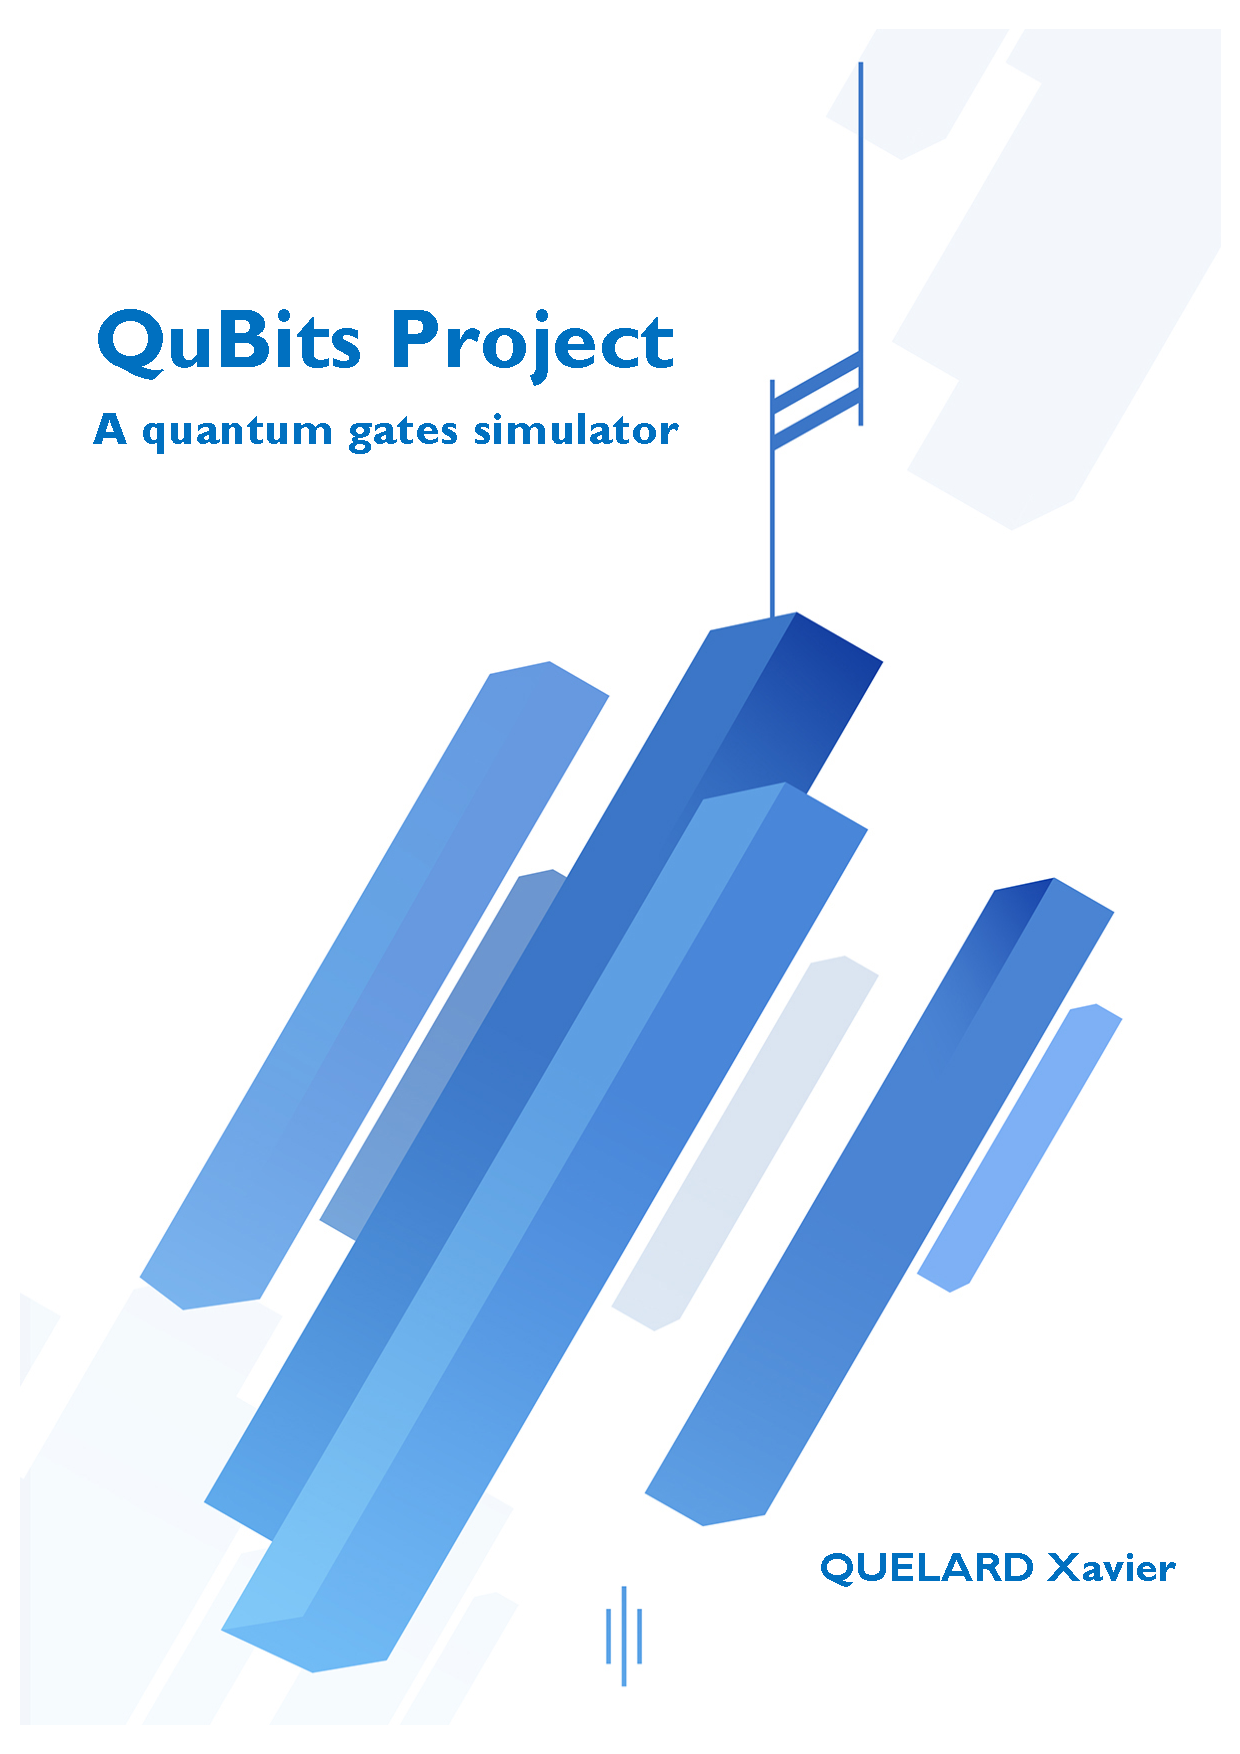
\includepdf{Garde}
\maketitle

\chapter*{Résumé}

\para{
	...
}

\tableofcontents

\chapter*{Introduction}
\addcontentsline{toc}{chapter}{Introduction}

\para{
	...
}

\chapter{Historique : mécanique quantique et QuBit}

\para{
	...
}

\chapter{Comment réaliser un QuBit?}
	\section{Photons polarisés}

\para{
	...
}

	\section{Pièges à ions / technologie NMR}

\para{
	...
}

	\section{Pièges à ions / technologie NMR}

\para{
...
}

	\section{Solid State QuBit (supraconductor technology)}

\para{
...
}

\chapter{Simulation informatique}
	\section{Rappels mathématiques}
		\subsection{Loi de composition interne et groupe}

\par{
Une loi de composition interne $\star{}$ sur l'ensemble $X$ est une aplication de la forme : \[\star : X \times X \rightarrow X\]
}

\par{
	Soit $G$ un ensemble non vide, muni d'une loi de composition interne \oplus. $ (G, \oplus)$ est un groupe abélien \Leftrightarrow
}

\begin{itemize}
\item[$\bullet$] $\oplus$ associative : $\forall (x,y) \in G^2, (x \oplus y) \oplus y = x \oplus ( y \oplus z )$
\item[$\bullet$] $\exists e \in G / x \oplus e = e \oplus x = x$ (e est le neutre du groupe G selon la loi $\oplus$)
\item[$\bullet$] $\oplus$ commutative : $\forall (x,y) \in G^2, x \oplus y = y \oplus x$ \\
\end{itemize}

		\subsection{Anneaux et corps}

\par{
	Disposant de la définition d'un corps commutatif, nous pouvons maintenant donner la définition d'un anneau commutatif. Soit $A$ un ensemble non vide, muni de deux lois de compositions interne \oplus et \otimes.
}

\par{
	Alors $(A, \oplus, \otimes)$ anneau commutatif $\Leftrightarrow$
}

\begin{itemize}
\item[$\bullet$] $ (A, \oplus)$ est un groupe commutatif
\item[$\bullet$] la loi $\otimes$ est associative
\item[$\bullet$] la loi $\otimes$ est distributive par rapport à la loi $\oplus$, c'est-à-dire que : \[ \forall (x,y,z) \in A^3, (x \oplus y) \otimes z = x \otimes ( y \oplus z ) \]
\item[$\bullet$] la loi $\otimes$ est commutative : $\forall (x1,x2) \in A^2, x1 \otimes x2 = x2 \otimes x1$
\end{itemize}

\vspace{1\baselineskip}

\par{
	Un corps commutatif est alors simplement un anneau commutatif dont tous les éléments sont inversibles, exceptés le neutre pour l'opération $\oplus$. Il est alors aisé de remarquer que l'ensemble $\mathbb{R}$ ou bien $\mathbb{C}$ sont, munis des opérations $(+,\times)$, des corps.
}

		\subsection{espace vectoriel et produit scalaire}

\par{
	Soit $E$ un ensemble non vide et $(\mathbb{K},+,\times)$ un corps de neutre $0_{\mathbb{K}}$ pour $+$ et $1_{\mathbb{K}}$ pour $\times$. On note $(E,+,\cdot)$ l'ensemble $E$ muni de la même loi $+$ que $\mathbb{K}$ (c'est donc une loi interne à $E$), et d'une loi externe $\cdot : \mathbb{K} \times E \rightarrow E$ .
}

\par{
	Alors $E$ est un espace vectoriel $\Leftrightarrow$
}

\begin{itemize}
\item[$\bullet$] $ (E, +)$ est un groupe commutatif
\item[$\bullet$] $\forall \lambda \in \mathbb{K}, \forall (x,y) \in E^2, \lambda \cdot (x+y) = (\lambda \cdot x) + (\lambda \cdot y)$ (distributivité)
\item[$\bullet$] $\forall (\lambda, \mu) \in \mathbb{K}^2, \forall x \in E, (\lambda + \mu) \cdot x = \lambda \cdot x + \mu \cdot x$
\item[$\bullet$] $\forall (\lambda, \mu) \in \mathbb{K}^2, \forall x \in E, (\lambda \times \mu) \cdot x = \lambda \cdot (\mu \cdot x)$
\item[$\bullet$] $\forall x \in E, 1_{\mathbb{K}} \cdot x = x$
\end{itemize}

\vspace{1\baselineskip}

\par{
	On appele les éléments de $E$ des vecteurs, les éléments de $\mathbb{K}$ des scalaires, et le vecteur $0_{\mathbb{K}}$ est appelé le vecteur nul. En résumé, un espace vectoriel est un espace E consitué d'éléments appelés vecteurs, qui sont stables par addition et par multiplication d'un scalaire. Les espaces $(\mathbb{R},+,\cdot)$ et $(\mathbb{C},+,\cdot)$ sont donc des espaces vectoriels (le second est appelé espace vectoriel complexe).
}

\vspace{1\baselineskip}

\par{
	On appele produit scalaire sur $E$ (espace vectoriel) toute forme bilinéaire symétrique et définie positive, c'est-à-dire :
}

\begin{itemize}
\item[$\bullet$] forme : c'est une application du type
$\prodSc{\cdot}{\cdot} : \left\{
  \begin{array}{rcr}
    E \times E \rightarrow \mathbb{K} \hfill \\
    (u,v) \mapsto \langle u / v \rangle \\
  \end{array}
\right$
\item[$\bullet$] symétrie : $ \forall (u,v) \in E^2, \prodSc{u}{v} = \prodSc{v}{u} $
\item[$\bullet$] linéarité (de la symétrie découle alors la bi-linéarité) : $\forall (u,v,w) \in E^3, \proSc{u}{v+w}= \prodSc{u}{v} + \prodSc{u}{w}$
\item[$\bullet$] defini positif : $\forall u \in E, \proSc{u}{u} \geq 0$ et $\forall u \in E, \prodSc{u}{u} = 0 \Lefrightarrow u = 0_{E}$
\end{itemize}

\vspace{1\baselineskip}

\par{
	Il est important de remarquer que s'il l'on se place dans un espace vectoriel complexe, le produit scalaire donne un nombre complexe, tandis qu'en se plaçant dans un espace vectoriel sur le corps des réels, le produit scalaire donnera lui même un réel. De manière générale, il associe à vecteur un élément du corps $\mathbb{K}$.
}

		\subsection{norme induite, suites de Cauchy et espace de Hilbert}

\par{
	Une norme est une application $N : E \rightarrow \mathbb{R}_{+}$ et qui satisfait l'hypothèse de séparation ($\forall u \in E, N(u) = 0 \Rightarrow u = 0_{E}$), d'absolue homogénéité ($\forall \lambda \in \mathbb{K}, \forall u \in E, N(\lambda \cdot u) = \lambda \cdot N(u)$), et l'inégalité triangulaire ($\forall (u,v) \in E^2, N(u+v) \leq N(u) + n(v)$).
}

\vspace{1\baselineskip}

\par{
	A chaque produit scalaire est associé une norme, que l'on appele norme induite par le produit scalaire. Elle est définie par :
}

\begin{equation}
N( \cdot ) : \left\{
  \begin{array}{rcr}
    E \rightarrow \mathbb{R}_{+} \hfill \\
    u \mapsto \sqrt{\prodSc{u}{u}} \\
  \end{array}
\right
\end{equation}

\vspace{1\baselineskip}

\par{
	Une fois que nous possédons une norme, il est possible d'introduire la notion de convergence, mais aussi de définir les suites de Cauchy. Soit $(U)_{n}$ une suite de vecteurs de $E$. Alors $(U)_{n}$ suite de Cauchy $\Leftrightarrow$
}

\begin{equation} \forall \varepsilon \in \mathbb{R}_{+}^*, \exists N \in \mathbb{N} / \forall (p,q) \in \mathbb{N}^2, |u_{p} - u_{q}| < \varepsilon  \end{equation}

\par{
	Une suite de Cauchy est donc simplement une suite dont les termes se rapprochent uniformément les uns des autres en l'infini. Un espace vectoriel, muni d'une norme découlant d'un produit scalaire, et dont toutes les suites de Cauchy convergent, est appelé un espace de Hilbert. La convergence d'une suite vers une valeur $l \in \mathbb{K}$ se traduit par la propriété (\ref{convergence}) .
}

\begin{equation} \label{convergence} \forall \varepsilon \in \mathbb{R}_{+}^*, \exists N \in \mathbb{N} / \forall n \in \mathbb{N}, n \geq N \Rightarrow |u_{n} - l| < \varepsilon  \end{equation}

\vspace{1\baselineskip}

\par{
	C'est dans un tel espace que nous allons travailler pour définir nos QuBits.
}

	\section{Application aux QuBits ( + sphere de bloch)}

		\subsection{Définition d'un QuBit}

\par{
	Notons dans toute la suite $\mathbb{H}_{n}$ un espace de Hilbert complexe et de dimension $n$. Un vecteur quelconque de l'espace $\mathbb{H}_{2}$ est donc défini par : $\quSt{\Phi} = \lambda \quSt{0} + \mu \quSt{1}$, où $\lambda$ et $\mu$ sont des coefficient complexes, et où $\quSt{0}$ ainsi que $\quSt{1} $ sont deux vecteurs formant une base orthonormée de $\mathbb{H}_{2}$ (les deux vecteurs sont orthogonaux et de norme 1). Le produit scalaire de deux vecteurs est alors défini par \ref{prodScH2}), et la norme induite sera (\ref{normeH2}).
}

\begin{equation} \label{prodScH2}
	 \prodSc{\Phi}{\Psi} = \langle ~ \lambda \quSt{0} + \mu \quSt{1} ~/~ \nu \quSt{0} + \sigma \quSt{1} ~\rangle = \lambda^* \nu + \mu^* \sigma = \prodSc{\Phi}{\Psi}^*
\end{equation}

\begin{equation} \label{normeH2}
	 || \Phi ||^2 = \prodSc{\Phi}{\Phi} = \langle ~ \lambda \quSt{0} + \mu \quSt{1} ~/~ \lambda \quSt{0} + \mu \quSt{1} ~\rangle = |\lambda|^2 + |\mu|^2
\end{equation}

\vspace{1\baselineskip}

\par{
	Un QuBit isolé est alors défini comme un vecteur de cet espace $\mathbb{H}_{2}$ (voir \ref{QuBit} ) auquel on ajoute une conditionsur la norme : la condition de normalisation (\ref{normalisation}). Si cette dernière n'est pas indispensable, elle est commode et constamment utilisé dans la littérature, nous l'adopterons donc également.
}

\begin{equation} \label{QuBit}
	\quSt{Q} = \alpha \cdot \quSt{0} + \beta \cdot \quSt{1}
\end{equation}

\begin{equation} \label{normalisation}
	(\alpha,\beta) \in \mathbb{C}^2 / |\alpha|^2 + |\beta|^2 = 1
\end{equation}

		\subsection{QuBit et mesure}

\par{
	La mesure d'un QuBit corresponds à une application $\mathbb{M} : \mathbb{H}_{2} \rightarrow \{ \quSt{0}, \quSt{1} \}$ : on prends un QuBit et on détermine si ce dernier "était" dans l'état $\quSt{0}$ ou $\quSt{1}$. Mais comme vu dans la première partie de ce rapport, la mesure en mécanique quantique n'est pas une chose exacte : en effet, si le QBit était de la forme $\quSt{Q} = \quSt{0}$, et que l'on mesure la probabilité que ce dernier soit dans l'état $\quSt{0}$, nous obtiendrons bel et bien 100\%. De même, si $\quSt{Q} = \quSt{1}$, nous obtiendrons une probabilité de 0\%. En revanche, dans le cas général, tout se complique. Soit $\quSt{\omega}$ un vecteur de $\mathbb{H}_{2}$. Nous voulons connaître la probabilité selon laquelle notre QuBit sera mesuré dans l'état $\quSt{\Omega}$. Elle est définie par (\ref{probaState}).
}

\begin{equation} \label{probaState}
	P(~ M( \quSt{Q} ) = \quSt{\Omega} ~) = | \langle ~ \quSt{Q} ~/~  \quSt{\Omega} ~\rangle |^2 = P(~ M( Q ) = \Omega ~)
\end{equation}

\vspace{1\baselineskip}

\par{
	La conséquence logique des dernières affirmations est que pour un QuBit de la forme $\quSt{Q} = \alpha \cdot \quSt{0} + \beta \cdot \quSt{1}$, ses probbilités d'être mesuré dans l'état $\quSt{0}$ est de $\lambda^2$, et celle d'être mesuré dans l'état $\quSt{1}$ est de $\mu^2$. la condition de normalisation (\ref{normalisation}) prends alors tout son sens : la somme des probabilités de deux évènements formant un ensemble complet vaut 1. Ce résultat se généralise pour n'importe quel couple d'etats , tant que ces derniers forment une base orthonormée.
}

		\subsection{Visualisation avec la sphère de Bloch}

\par{
	L'objectif de cette section est de donner un aperçu visuel au lecteur d'un état quantique. C'est à cette problématique que la sphère de Bloch, nommée après le brillant mathématicien, apporte une réponse. Pour présenter cette dernière, il est d'abord nécessaire de définir les relations et classes d'équivalences. \\
	%$\bm{\lambda = \prodSc{Q}{0} }$ \\ \\ $\bm{\mu = \prodSc{Q}{1}}$ \\ \\ $\bm{\quSt{Q}~\quSt{0}~\quSt{1}}$
}

\par{
	$R : E \rightarrow E  $ relation d'équivalence \Leftrightarrow
}

\begin{itemize}
\item[$\bullet$] $R$ refléxive : $\forall x \in E, x R x$ (x est en relation avec lui même)}
\item[$\bullet$] $R$ symétrique : $\forall (x,y) \in E^2, x R y \Rightarrow y R x$
\item[$\bullet$] $R$ transitive : $\forall (x,y,z) \in E^3, x R y \text{ et } y R z \Rightarrow x R z$
\end{itemize}

\vspace{1\baselineskip}

\par{
	Une classe d'équivalence d'un élément $x$, notée $[x]$, est alors simplement défini comme le sous ensemble de E contenant tous les éléments de E en relation avec x, soit plus formellement : $x \in E, \forall y \in E, y \in [x] \Leftrightarrow y R x$ . Avec ceci en tête, examinons maintenant la relation $R : \mathbb{H}^2 \rightarrow \mathbb{H}^2$
}

\begin{equation}
	 \quSt{\Psi} R \quSt{\Psi '} \Leftrightarrow \exists z \in \mathbb{C} / \left\{
		  \begin{array}{rcr}
		      \quSt{\Psi} R \quSt{\Psi '} \Leftrightarrow \quSt{\Psi} = z \quSt{\Psi '} \\
		      |z| = 1 \\
		  \end{array}
		\right
\end{equation}

\vspace{1\baselineskip}

\par{
	$R$ est une relation d'équivalence (la réfléxivité, la symétrie et la transitivité sont toutes trivialement vérifiées). Deux QuBit appartenant à une même classe d'équivalence sont égaux, à une multiplication par un complexe $z$ de module 1. Un tel $z = e^{i\theta}$ est appelé un facteur de phase. Un QuBit pur est alors simplement un représentant d'une classe d'équivalence de la relation d'équivalence évoquée ci-dessus. Multiplier un état par un facteur de phase ne changera par la probabilité d'être mesuré dans un état $\quSt{\alpha}$ donné. En effet :
}

\begin{align}
	P(~ M( z \quSt{\Psi} ) = \quSt{\alpha} ~) &= \prodSc{z \quSt{\Psi}}{\quSt{\alpha}} \\
	 &= |z| \prodSc{\quSt{\Psi}}{\quSt{\alpha}} \\
	 &= P(~ M( \quSt{\Psi} ) = \quSt{\alpha} ~)
\end{align}

\vspace{1\baselineskip}

\par{
	On peux alors supposer que deux vecteurs de $\mathbb{H}^2$ sont équivalents s'ils ne différent que par un facteur de phase, ce qui amène à la réécriture suivante :
}

\begin{align}
	\label{blochEq}
	\forall \quSt{\Psi} \in \mathbb{H}^2 , \exists \theta \in [0, \pi] ~/~ \quSt{\Psi} &= \cos(\theta/2) \cdot \quSt{0} + \sin(\theta/2) e^{i(\varphi)} \cdot \quSt{1} \\
	&\equiv \cos(\theta/2) e^{-i(\varphi/2)} \cdot \quSt{0} + \sin(\theta/2) e^{i(\varphi/2)} \cdot \quSt{1}
\end{align}

\vspace{1\baselineskip}

\para{
Sous cette nouvelle forme, il est possible de représenter tout QuBit pur comme point sur une sphère, où $\theta$ et $\varphi$ font office de colatitude et longitude (voir figure \ref{bloch}). La correspondance entre l'espace des QuBit purs et une sphère de Bloch est un isomorphisme : une application bijective entre deux espaces, dont la réciproque est également bijective. On constate cependant sur la figure \ref{bloch} que la linéarité n'est pas préservée (en effet, $\quSt{0} \neq -\quSt{1}$). Il faut ainsi considérer cette relation comme une occasion de visualiser plus simplement l'état des QuBits, mais ne permettant pas nécessairement d'interprétations graphiques cohérentes.
}

\begin{figure}
	\begin{center}
		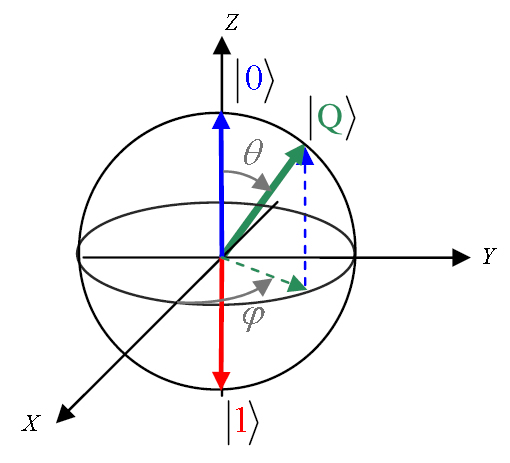
\includegraphics[scale=0.60]{images/bloch}
	\end{center}
	\caption{\textit{Visualisation d'un état quantique dans la sphère de Bloch.}}
	\label{bloch}
\end{figure}

		\subsection{extension à plusieurs QuBits}

\para{
	Le passage de un à deux QuBit apporte de nombreuses nouveautés et dévoile une complexité qui pourrait sembler à priori innatendue. Mais c'est cette dernière qui donne tout son potentiel à l'informatique quantique. Pour expliquer ce dernier, il est nécessaire de définir le produit tensoriel $\otimes$ de deux QuBits (\ref{tensoriel}) .
}

\begin{equation}
	\label{tensoriel}
	(\cdot) \otimes (\cdot) : \left\{
	  \begin{array}{rcr}
	    \mathbb{H_1}^2 \times \mathbb{H_2}^2 \rightarrow \mathbb{H}^4 \hfill \\
	    (\quSt{\varphi},\quSt{\Psi}) \mapsto \quSt{\varphi} \otimes \quSt{\Psi} = \left( \begin{array}{c} \alpha \\ \beta \\\end{array} \right ) \otimes \left( \begin{array}{c} \lambda \\ \mu \\ \end{array} \right ) = \left( \begin{array}{c} \alpha \lambda \\ \alpha \mu \\ \beta \lambda \\ \beta \mu \end{array} \right ) \\
	  \end{array}
	\right
\end{equation}

\para{
	Le produit tensoriel de deux espaces $\mathbb{H_i}^2$, qui corresponds à l'espace dans lequel deux QuBits existent, est défini par un espace dont la base est égale à toutes les combinaisons possibles de produit tensoriels entre les vecteurs de bases des deux espaces de départ. C'est donc un espace de dimension 4 ayant pour base orthonormée :
}

\begin{equation}
	 \{ \quSt{0_A \otimes 0_B}, \quSt{0_A \otimes 1_B} , \quSt{1_A \otimes 0_B} , \quSt{1_A \otimes 1_B} \} = \{ \quSt{00}, \quSt{01}, \quSt{10}, \quSt{11} \}
\end{equation}

\begin{equation}
	 =  \left\{ \left( \begin{array}{c} 1 \\ 0 \\ 0 \\ 0 \end{array} \right ), \left( \begin{array}{c} 0 \\ 1 \\ 0 \\ 0 \end{array} \right ), \left( \begin{array}{c} 0 \\ 0 \\ 1 \\ 0 \end{array} \right ), \left( \begin{array}{c} 0 \\ 0 \\ 0 \\ 1 \end{array} \right ) \right\} \\
\end{equation}

\vspace{1\baselineskip}

\begin{equation}
	 =  \left\{ \left( \begin{matrix} 1 & 0 \\ 0 & 0 \end{matrix} \right ), \left( \begin{matrix} 0 & 1 \\ 0 & 0 \end{matrix} \right ), \left( \begin{matrix} 0 & 0 \\ 1 & 0 \end{matrix} \right ), \left( \begin{matrix} 0 & 0 \\ 0 & 1 \end{matrix} \right ) \right\} \\
\end{equation}

\vspace{1\baselineskip}

\par{
	On définit les états quantiques purs comme étant ceux pouvant s'écrire $\quSt{\varphi} \otimes \quSt{\Psi}$. En reprenant les coefficients utilisés dans l'equation (\ref{tensoriel}), on en déduit que les états quantiques purs sont ceux de la forme :
}

\begin{equation}
	\quSt{\varphi} \otimes \quSt{\Psi} = \alpha \lambda \cdot \quSt{00} + \alpha \mu \cdot \quSt{01} + \beta \lambda \cdot \quSt{10} + \beta \mu \cdot \quSt{11}
\end{equation}

\vspace{1\baselineskip}

\par{
	Les états quantiques n'étant pas purs sont dits intriqués, et l'existence de ces derniers a remis en cause le principe de localité que nous avons évoqués dans la partie 1. En effet, si l'on considère l'état de Bell : $\quSt{\Psi} = \frac{1}{\sqrt{2}} \cdot (~ \quSt{00} + \quSt{11}  ~)$. Alors une mesure de l'un des deux QuBit dans sa base respective nous donnera immédiatement l'information de la mesure du second QuBit dans sa propre base, même si les deux QuBit, après intrication, sont séparés d'un potentielle très grande distance\footnote{Des tests expérimentaux confirme cet effet pour une distance supérieure à 10km.}.
}

\vspace{1\baselineskip}

\par{
	Il semblerait tentant de faire un parallèle à l'informatique classique : deux bits peuvent ainsi former un registre dans seulement 4 états possibles : ${ 00, 01, 10, 11 }$. Cependant, là où il n'y a que quatre possibilités fixes en informatique classiques, il est nécessaire de se rappeler que dans $\mathbb{H}^4$, les vecteurs / registres de deux QuBits sont des combinaisons linéaires des vecteurs $ \{ \quSt{00}, \quSt{01}, \quSt{10}, \quSt{11} \} $. Les possibilités sont donc immenses, et tant qu'aucune mesure n'est effectuée, l'état quantique est maintenu (nous ne reparlerons par ici des problèmes de décohérence présentés en partie 1), conservant ainsi l'incertitude qui fait la force de l'informatique quantique. Ainsi, chaque ajout de QuBit augmente exponentiellement le nombre de combinaisons possibles comparées aux combinaisons "classiques".
}

	\section{Portes logiques}

		\subsection{évolution dans le temps d'un QuBit}

\par{
	Les relations établies dans les parties précédentes ont été écrites dans un espace $\mathbb{H}^2$ concernant un unique QuBit, puis généralisées à un ensemble de deux QuBit. Le passage à un nombre supérieur de QuBit s'effectuera exactement de la même manière, avec le produit tensoriel, défini de manière légèrement plus généralisée, pour pouvoir s'appliquer à deux espaces $\mathbb{H1}$ et $\mathbb{H2}$ de dimension quelconque.
}

\vspace{1\baselineskip}

\par{
	Nous pouvons donc désormais considérer un état quantique appartenant à un espace $\mathbb{H}^{2^n}$ , c'est-à-dire un registre composé de n QuBits. Notons cet espace plus simplement $\mathbb{H}^{\otimes n}$. Il est alors possible de donner l'équation de Schrödinger, qui décrit l'évolution dans le temps de tout état quantique précédant une mesure par :
}

\begin{equation}
	\frac{d \Psi(t)}{dt} = -i H \Psi(t)
\end{equation}

\vspace{1\baselineskip}

\par{
	Où $H$ est l'opérateur Hamiltonien. Dans ce cas particulier de la résolution de l'équation de Schrödinger (pour l'instant, j'ai du mal à comprendre parfaitement d'où sortent les hypothèses menant aux simplifications donnant l'equation ci-dessus), nous avons tout simplement une solution de la forme $\Psi(t) = U(t) \Psi(0)$, où $U(t) = e^{-itH}$. Notons que cette évolution temporelle ne modifie pas la norme de l'état quantique $\Psi$.
}

		\subsection{algèbre des portes logiques}

\par{
	Faire fonctionner un ordinateur classique requiert de savoir créer des bits (de nos jours, il s'agit de transistors de quelques dizaines de nanomètres), mais également de pouvoir utiliser des opérations sur ces derniers. Ainsi, avec des portes NOT, AND, OR, XOR etc, il est possible de fabriquer toutes les opérations indispensables à un algèbre de base, donnnant ainsi à l'ordinateur une grande puissance de calcul.
}

\vspace{1\baselineskip}

\par{
	L'analogie avec l'ordinateur quantique est parfaitement justifiée : il nous faut créer des portes logiques quantiques pouvant agir sur des QuBits afin de pouvoir faire d'un ordinateur quantique une réalité. De manière générale, une porte logique est une application de la forme :
}

\begin{align}
	\label{porteLogique}
	L( ... ) : \left\{
	  \begin{array}{rcr}
	    \mathbb{H}^{\otimes n} \times \mathbb{H}^{\otimes n} \times \mathbb{H}^{\otimes n} \times ... &\rightarrow \mathbb{H}^{\otimes n} \times \mathbb{H}^{\otimes n} \times \mathbb{H}^{\otimes n} \times ... \hfill \\
	    (\quSt{\varphi }, \quSt{\Psi }, \quSt{\Omega }, ... ) &\mapsto (L(\varphi),L(\Psi),L(\Omega), ...) \\
	  \end{array}
	\right
\end{align}

\par{
	C'est donc simplement une application linéaire qui a un nombre donné de QuBit tous de même dimension, renvoi un même nombre de QuBits dans un état potentiellement différent. Une porte quantique n'effectuant pas de mesure, il est nécessaire que la transformation maintienne la condition de normalité. Au final, pour représenter une porte logique, il suffira d'utiliser une matrice $M$ de norme 1. L'état de chaque QuBit après passage dans $L$ sera ainsi facilement calculé par $L(\Psi) = M \cdot \Psi$ . Par définition, il apparait que le calcul quantique est spontanément réversible.
}

		\subsection{portes logiques à 1 QuBit}

\par{
	Nous allons maintenant nous intéresser à plusieurs portes quantiques classiques, en commençant bien sur par le niveau le plus bas : les portes agissant sur un registre d'un seul QuBit. Nous allons définir deux porte quantiques, phase $L_{\Phi}$ et rotation $L_{\alpha}$, à partir desquelles il est possible de reconstruire toutes les portes de "dimension 1". Notons $Mat()$ l'application qui à une porte quantique associe l'unique matrice la représentant (on se positionne dans la base orthonormée $\{ \quSt{0}, \quSt{1} \}$). Alors :
}

\begin{equation}
	 Mat(L_{\Phi}) = \left( \begin{matrix} 1 & 0 \\ 0 & e^{i\Phi} \end{matrix} \right ) \\
\end{equation}

\begin{equation}
	 Mat(L_{\alpha}) = \left( \begin{matrix} cos(\alpha) & sin(\alpha) \\ -sin(\alpha) & cos(\alpha) \end{matrix} \right ) \\
\end{equation}

\vspace{1\baselineskip}

\par{
	La première porte ajoute un vecteur de phase à $\quSt{1}$, tandis que la seconde effectue une rotation de $\alpha$ du QuBit. Ces transformations rappellent exactement la définition d'un point sur la sphère de Bloch (equation \ref{blochEq}), ce qui nous permet d'affirmer qu'il est effectivement possible d'aboutir à n'importe quelle transformation à partir de ces deux portes logiques. On peux ainsi définir la classique porte NOT (négation du QuBit) et la porte de Hadamard :
}

\begin{equation}
	 Mat(NOT) = \left( \begin{matrix} 0 & 1 \\ 1 & 0 \end{matrix} \right ) \\
\end{equation}

\begin{equation}
	 Mat(HADAMARD) = \frac{1}{\sqrt{2}} \left( \begin{matrix} 1 & 1 \\ 1 & -1 \end{matrix} \right ) \\
\end{equation}

\vspace{1\baselineskip}

\par{
	Si l'interprétation de la porte $NOT$ est immédiate, il convient de revenir rapidement sur la porte de $HADAMARD$. C'est une porte indispensable en programmation quantique: en effet, elle sert souvent de première étape lors d'un algorithme, pour faire passer un registre d'un état initial $\quSt{0}_i$ pour chacun de ses QuBit à un état final de superposition des $2^n$ états $\quSt{0}_i$ et $\quSt{1}_i$ de podération/norme égale à $\frac{1}{2}$.
}

		\subsection{portes logiques à 2 QuBit (j'ai choisi de pas parler de la porte CU)}

\par{
	Les portes logiques à deux QuBit suivent toutes une logique similaire : l'un des deux QuBit est appelé QuBit contrôle, et l'autre QuBit cible (usuellement, nous les "positionnons" dans cet ordre). L'idée est alors de contrôler l'état du QuBit de contrôle, et d'agir -ou non- sur le QuBit cible en fonction du résultat.
}

\vspace{1\baselineskip}

\par{
	Nous pouvons alors très facilement définir deux premières portes quantiques sur deux QuBits : la porte $CNOT$ qui appliquera ou non la transformation $NOT$ sur le QuBit cible, et la porte $CPHASE$ qui appliquera potentiellement une phase au QuBit ciblé. Enfin, la porte $SWAP$ va simplement échanger les composantes $\quSt{01}$ et $\quSt{}$. Voici leur matrices :
}

\begin{equation}
	 Mat(CNOT) = \left( \begin{matrix} 1 & 0 & 0 & 0 \\ 0 & 1 & 0 & 0 \\ 0 & 0 & 0 & 1 \\ 0 & 0 & 1 & 0 \\ \end{matrix} \right ) \\
\end{equation}

\vspace{1\baselineskip}

\begin{equation}
	 Mat(CPHASE) = \left( \begin{matrix} 1 & 0 & 0 & 0 \\ 0 & 1 & 0 & 0 \\ 0 & 0 & 1 & 0 \\ 0 & 0 & 0 & e^{i\Phi} \\ \end{matrix} \right ) \\
\end{equation}

\vspace{1\baselineskip}

\begin{equation}
	 Mat(SWAP) = \left( \begin{matrix} 1 & 0 & 0 & 0 \\ 0 & 0 & 1 & 0 \\ 0 & 1 & 0 & 0 \\ 0 & 0 & 0 & 1 \\ \end{matrix} \right ) \\
\end{equation}

		\subsection{Ensemble universel}

\par{
	Un ensemble universel est un ensemble de portes quantiques tel que tout calcul quantique soit décomposable en opération composées de ces différentes portes. Les ensembles $\{PHASE,ROTATION,CPHASE\}$ et $\{PHASE,ROTATION,CNOT\}$ (PREUVE?!) sont de tels ensembles universels. En effet, avec les deux premières portes, toute opération sur un unique QuBit est réalisable, tandis qu'avec la porte $CPHASE$ ou $CNOT$, une intrication est possible, ce qui permet de "descendre en dimension" et donc assurer que tout calcul est réalisable.
}

\chapter{Simulation d'algorithme quantiques}
	\section{Algorithme de Shor}
	\section{Algorithme de Grover}

%
% -----------------------
% [?] CONCLUSION
% -----------------------
%/

\chapter*{Conclusion}
\addcontentsline{toc}{chapter}{Conclusion}

\para{
	...
}

\chapter*{Bibliographie}

\para{
	...
}


\chapter*{Annexe}

\end{document}
